\documentclass{beamer}
\usepackage{multicol}
\usepackage[english]{babel} 
\usepackage{graphicx}
\usepackage{ragged2e}
\usepackage{geometry}
\usepackage{hyperref}
\justifying
\setbeamertemplate{caption}[numbered]

%\usetheme{AnnArbor}
%\usetheme{Antibes}
%\usetheme{Bergen}
%\usetheme{Berkeley}
%\usetheme{Berlin}
%\usetheme{Boadilla}
%\usetheme{boxes}
%\usetheme{CambridgeUS}
%\usetheme{Copenhagen}
%\usetheme{Darmstadt}
%\usetheme{default}
%\usetheme{Frankfurt}
%\usetheme{Goettingen}
%\usetheme{Hannover}
%\usetheme{Ilmenau}
%\usetheme{JuanLesPins}
%\usetheme{Luebeck}
%\usetheme{Madrid}
%\usetheme{Malmoe}
%\usetheme{Marburg}
%\usetheme{Montpellier}
%\usetheme{PaloAlto}
%\usetheme{Pittsburgh}
%\usetheme{Rochester}
%\usetheme{Singapore}
%\usetheme{Szeged}
\usetheme{Warsaw}

\title{Lecture 1 - Linear Regression}

%\subtitle{Optional Subtitle}

\author{Rodrigo Loza\inst{1}}

\institute[UCB]
{
  \inst{1}%
  Computational Biologist - pfm Medical\\
  Biomedical Engineer - Universidad Cat\'olica Boliviana "San Pablo" La Paz, Bolivia
}


\date{August, 2017}

\subject{Machine learning}

\begin{document}

\begin{frame}
  \titlepage
\end{frame}

\begin{frame}{Outline}
 \begin{multicols}{2}
  \tableofcontents
  \end{multicols}
\end{frame}

%%%%%%%%%%%%%%%%%%%%%%%%%%%%%%%%%%%%%%%% RESOURCES %%%%%%%%%%%%%%%%%%%%%%%%%%%%%%%%%%%%%%%
\section{Resources}
\subsection{books}
\begin{frame}{Resources}
\begin{flushleft}
Recommended books
\begin{itemize}
\justifying
\item Pattern Recognition and Machine Learning [Bis06]
\item Machine Learning: A Probabilistic Perspective [Mur12]
\item Machine Learning: The Art and Science of Algorithms That Make Sense of Data [Fla12] 
\end{itemize}
\end{flushleft}

\begin{flushright}
\begin{figure}
  \centering
    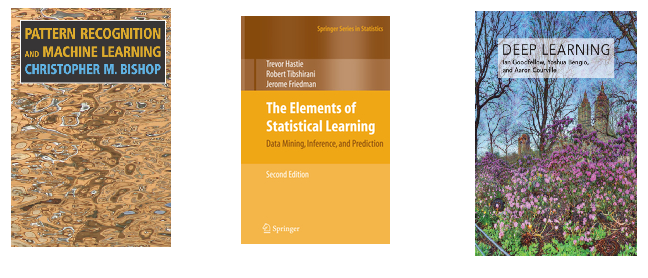
\includegraphics[width=0.55\textwidth]{books}
  		\caption{ Recommended books }
    \label{books}
 \end{figure}
\end{flushright}
\end{frame}

\subsection{Data Sets}
\begin{frame}{Data Sets}
\begin{figure}
  \centering
    
\includegraphics[width=0.75\textwidth]{datasets}
  		\caption{ Examples datasets }
    \label{books}
 \end{figure}
\end{frame}

%%%%%%%%%%%%%%%%%%%%%%%%%%%%%%%%%%%%%%%% Learning problem %%%%%%%%%%%%%%%%%%%%%%%%%%%%%%%%%%%%%%%
\section{Introduction}
\subsection{The learning problem}
\begin{frame}{Problem example}
\begin{figure}
  \centering
    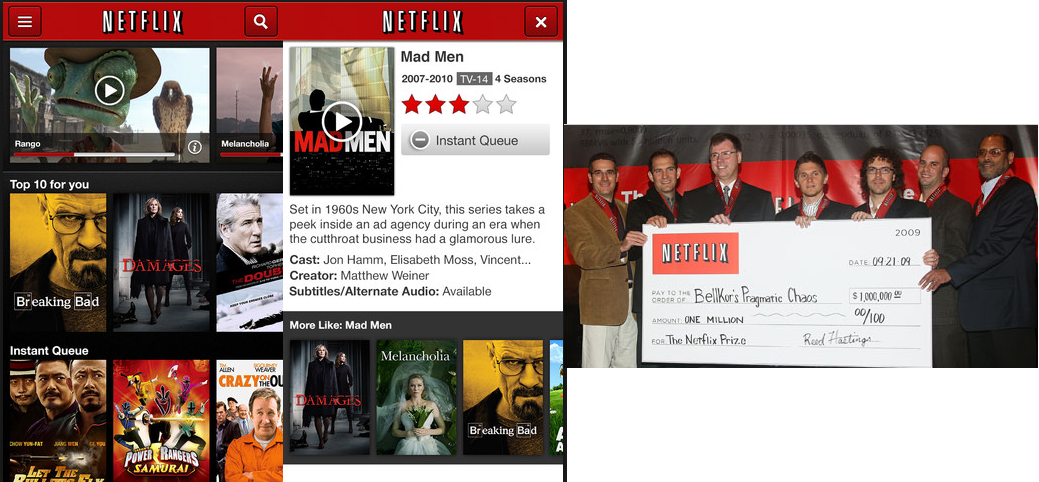
\includegraphics[width=0.75\textwidth]{netflixcomp}
  		\caption{ Netflix competition - recommendation systems }
    \label{netflix competition}
 \end{figure}
\end{frame}

\begin{frame}{Problem visualization}
\begin{figure}
  \centering
    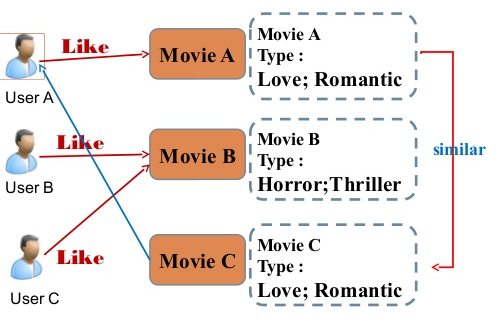
\includegraphics[width=0.75\textwidth]{movierecommendation}
  		\caption{ Visual way to describe the problem }
    \label{movie recommendation netflix}
 \end{figure}
\end{frame}

\begin{frame}{}
\textbf{Problem:} Predicting how a viewer will rate a movie \\
\textbf{10$\%$ improvement - 1 million dollars} \\
The essence of machine learning: 
\begin{enumerate}
\uncover<1->{\item A pattern exists}
\uncover<2->{\item There is no way to pin it down mathematically}
\end{enumerate}
\end{frame}

\begin{frame}{The components of learning}
Formalization: 
\begin{enumerate}
\uncover<1->{\item Input x: customer behaviour}
\uncover<2->{\item Output y: what movies does the customer like$?$}
\uncover<3->{\item Target function: f: x $-$ $>$ y}
\uncover<4->{\item Data: (x1,y1), (x2,y2), (x3,y3) ... (xn,yn)}
\uncover<5->{\item Hypothesis: g: x $-$ $>$ y}
\end{enumerate}
\end{frame}

\begin{frame}{Learning model}
\begin{figure}
  \centering
    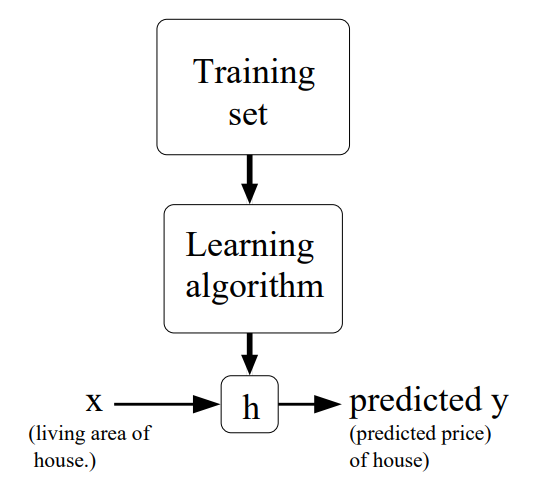
\includegraphics[width=0.45\textwidth]{learningalgorithm}
  		\caption{ Learning model }
    \label{lmodel}
 \end{figure}
\end{frame}

\begin{frame}{ Differences between a task and a learning model }
	”...tasks are addressed by models, whereas learning problems are \\ 
	solved by learning algorithms that produce models.”[Fla12]
  \begin{figure}
  \centering
    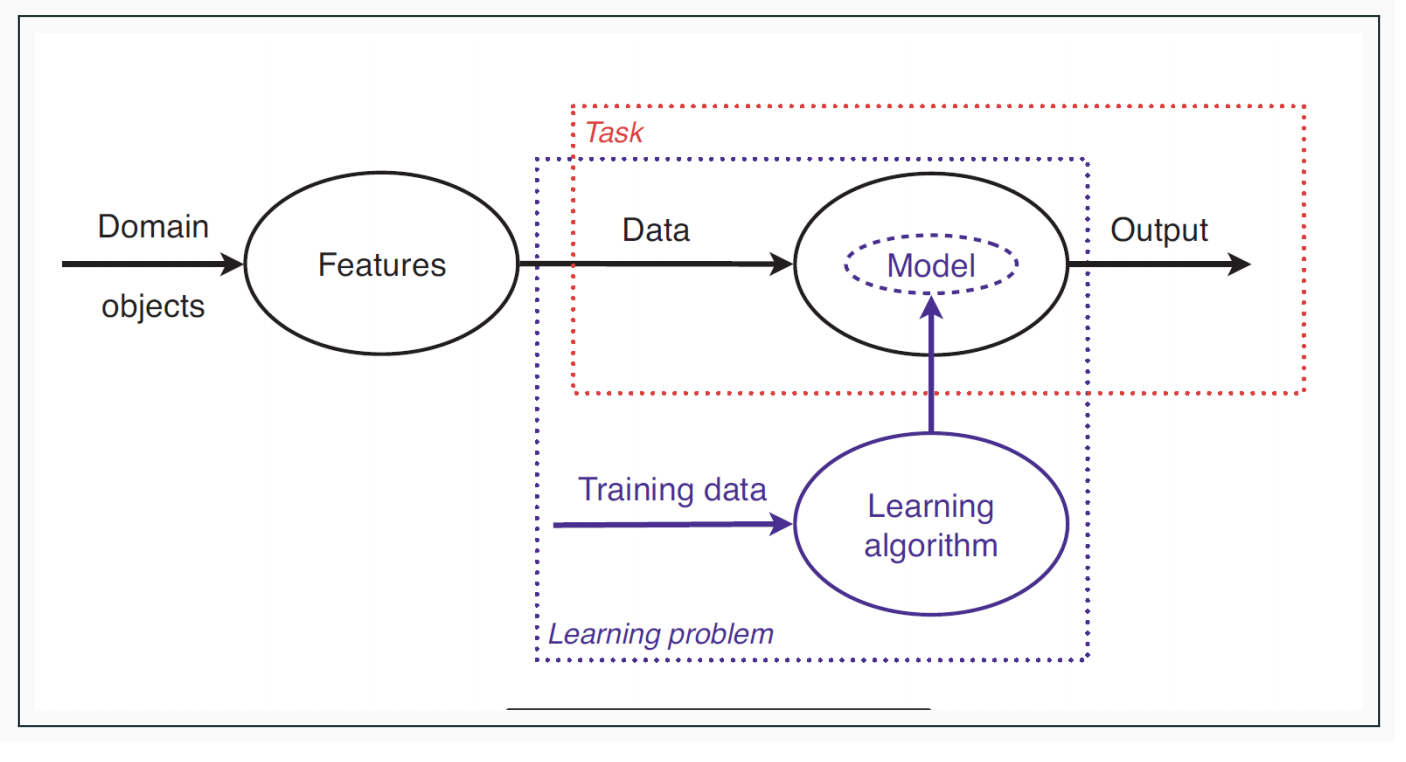
\includegraphics[width=0.65\textwidth]{addressingtask}
  		\caption{ Difference between a task and learning problems }
    \label{addressingtask}
 \end{figure}
\end{frame}

%%%%%%%%%%%%%%%%%%%%%%%%%%%%%%%%%%%%%%%% Machine learning %%%%%%%%%%%%%%%%%%%%%%%%%%%%%%%%%%%%%%%
\subsection{ML Definition}
\begin{frame}{What is Machine Learning?}
\begin{itemize}
\justifying
\item “Field of study that gives computers the ability to learn without
being explicitly programmed.” – Arthur Samuel, IBM, Stanford
University, 1959

\item “A computer program is said to learn from experience E with
respect to some task T and some performance measure P, if its
performance on T, as measured by P, improves with experience E.”
– Tom Mitchell [Mit97]

\item “Instead of writing a program by hand, we collect lots of examples
that specify the correct output for a given input. A machine
learning algorithm then takes these examples and produces a
program that does the job.” – Geoffrey Hinton [Hin14]
\end{itemize}
\end{frame}

\begin{frame}{ML is a subset}
\begin{figure}
  \centering
    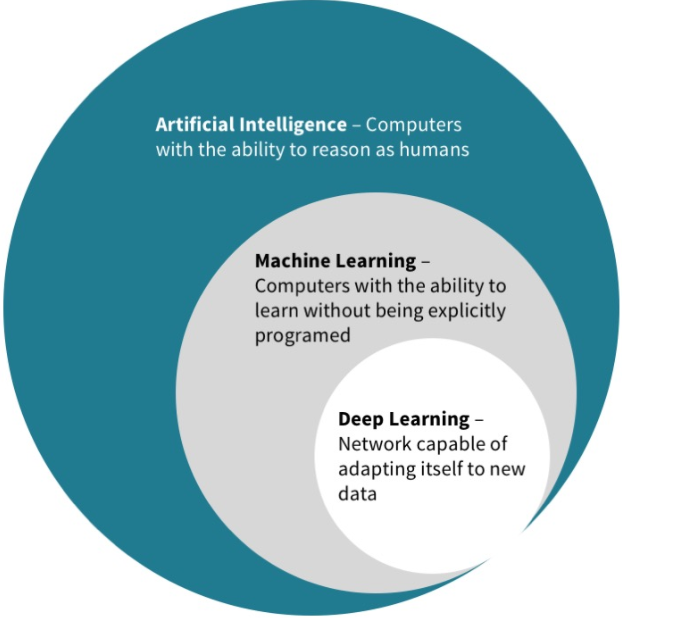
\includegraphics[width=0.65\textwidth]{mlsubset}
  		\caption{ Machine learning is a subset of parent sciences }
    \label{addressingtask}
 \end{figure}
\end{frame}

\begin{frame}{ ML solves problems with the following shape }
\begin{figure}
  \centering
    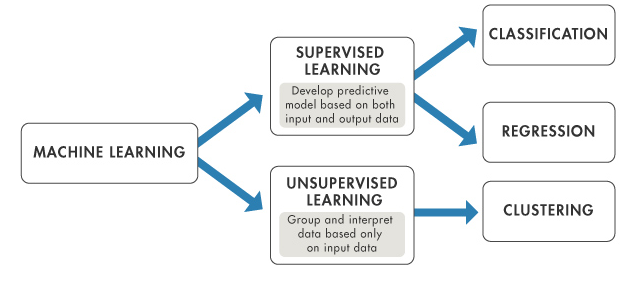
\includegraphics[width=0.65\textwidth]{mldivided}
  		\caption{ Types of problems machine learning solves }
    \label{addressingtask}
 \end{figure}
\end{frame}

\begin{frame}{ Supervised learning - probability interpretation }
\begin{figure}
  \centering
    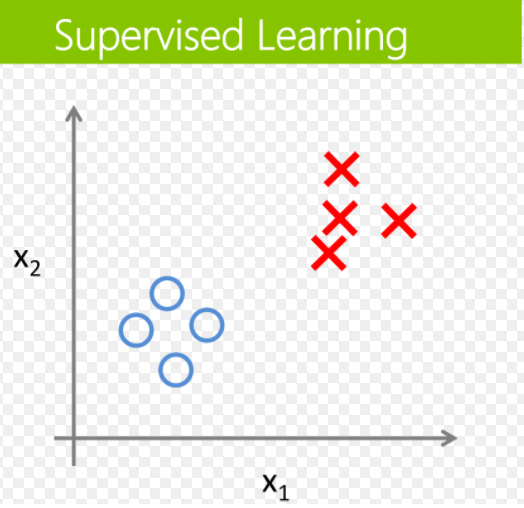
\includegraphics[width=0.65\textwidth]{supervised_learning}
  		\caption{ Supervised learning }
    \label{addressingtask}
 \end{figure}
\end{frame}

\begin{frame}{ Unsupervised learning - probability interpretation }
\begin{figure}
  \centering
    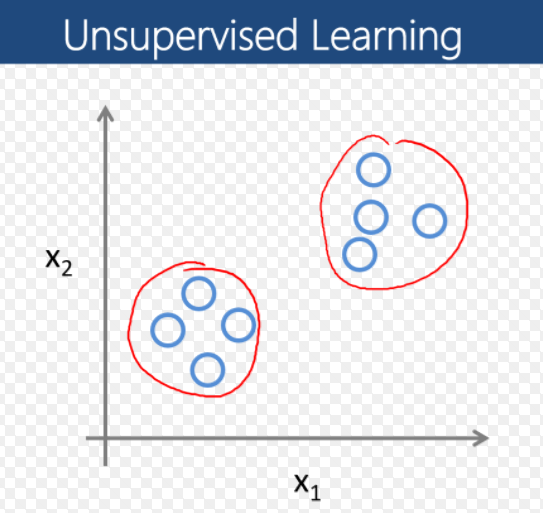
\includegraphics[width=0.65\textwidth]{unsupervised_learning}
  		\caption{ Unsupervised learning }
    \label{addressingtask}
 \end{figure}
\end{frame}

%%%%%%%%%%%%%%%%%%%%%%%%%%%%%%%%%%%%%Linear Regression%%%%%%%%%%%%%%%%%%%%%%%%%%%%%%%%%%%%%%%%%%%%%%%%%%%%%%%
%%%%%%%%%%%%%%%%%%%%%%%%%%%%%%%%%%%%%Univariate linear regression%%%%%%%%%%%%%%%%%%%%%%%%%%%%%%%%%%%%%%%
\section{Linear Regression}
\subsection{Linear Regression}
\begin{frame}{Definition}
\begin{itemize}
\item Model a single response \textbf{(dependent, continuous, outcome)} variable based on one or more input \textbf{(independent, predictor)} variables
\end{itemize}
\end{frame}

\begin{frame}{Linear Regression example}
\justify
\begin{itemize}
\item Suppose that we are given a training set comprising N observations of x,
written \textbf{x = (x1, ..., xn)} together with corresponding observations of the values
of y, denoted \textbf{y = (y1, ..., yn)}
\item The input data set x in Figure 1.2 was generated by choosing
values of xn, for n = 1,...,N, spaced uniformly in range [0, 1], and the target
data set t was obtained by first computing the corresponding values of the function sin(2pix)
\end{itemize}
\end{frame}

\begin{frame}{Linear Regression example}
\begin{figure}
  \centering
    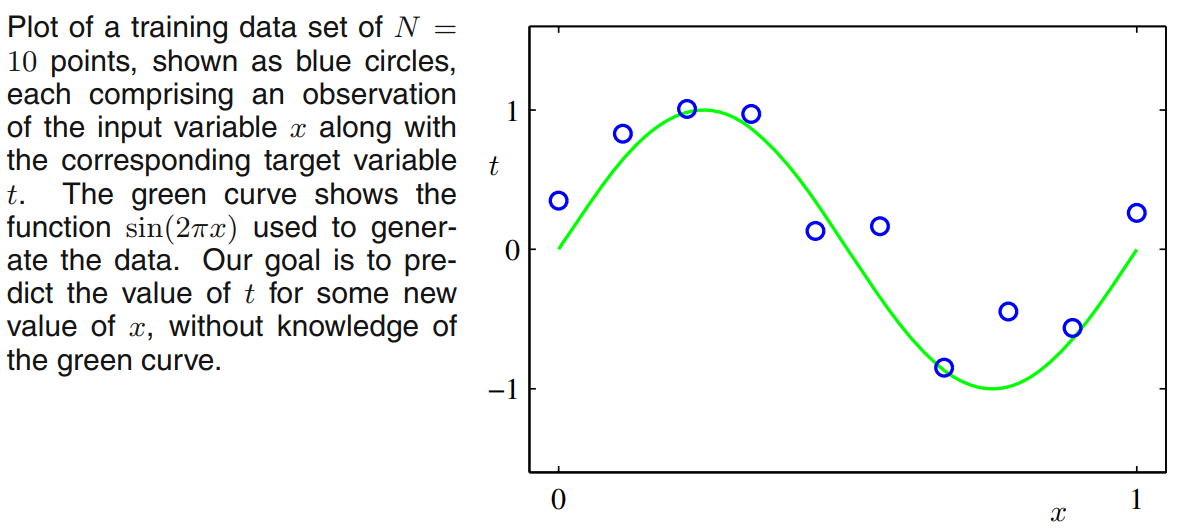
\includegraphics[width=0.75\textwidth]{sin2pix}
  		\caption{ Target function }
    \label{sinpix}
 \end{figure}
\end{frame}

\subsection{Hypothesis}
\begin{frame}{Curve fitting approach - Hypothesis}
We shall fit the data using a polynomial function of the form: \\
\begin{figure}
  \centering
    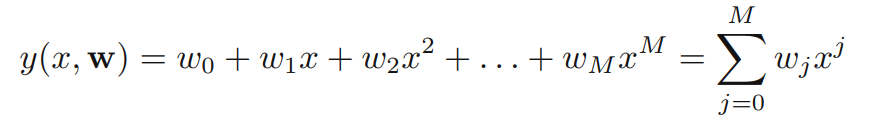
\includegraphics[width=0.80\textwidth]{hypothesis}
  		\caption{ Linear combination of learning parameters and features }
    \label{hypothesis}
 \end{figure}
\end{frame}

\subsection{Cost function}
\begin{frame}{Curve fitting approach - Cost function}
The values of the coefficients will be determined by fitting the polynomial to the training data. This can be done by minimizing an \textbf{error function} that meaures the misfit between the function \textbf{y(x, w)}, for any given value of w, and the training set data points. The simplest error function is the \textbf{sum of squares} of the errors between the predictions \textbf{y(xn, w) for each data point xn and the corresponding target values yn, so that we minimize: }  \\
\begin{figure}
  \centering
    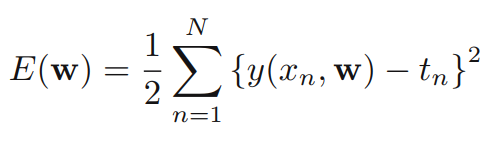
\includegraphics[width=0.60\textwidth]{cost_function}
  		\caption{ Cost function for continuous type variables }
    \label{cost_function}
 \end{figure}
\end{frame}

\begin{frame}{Curve fitting approach - Cost function}
\begin{figure}
  \centering
    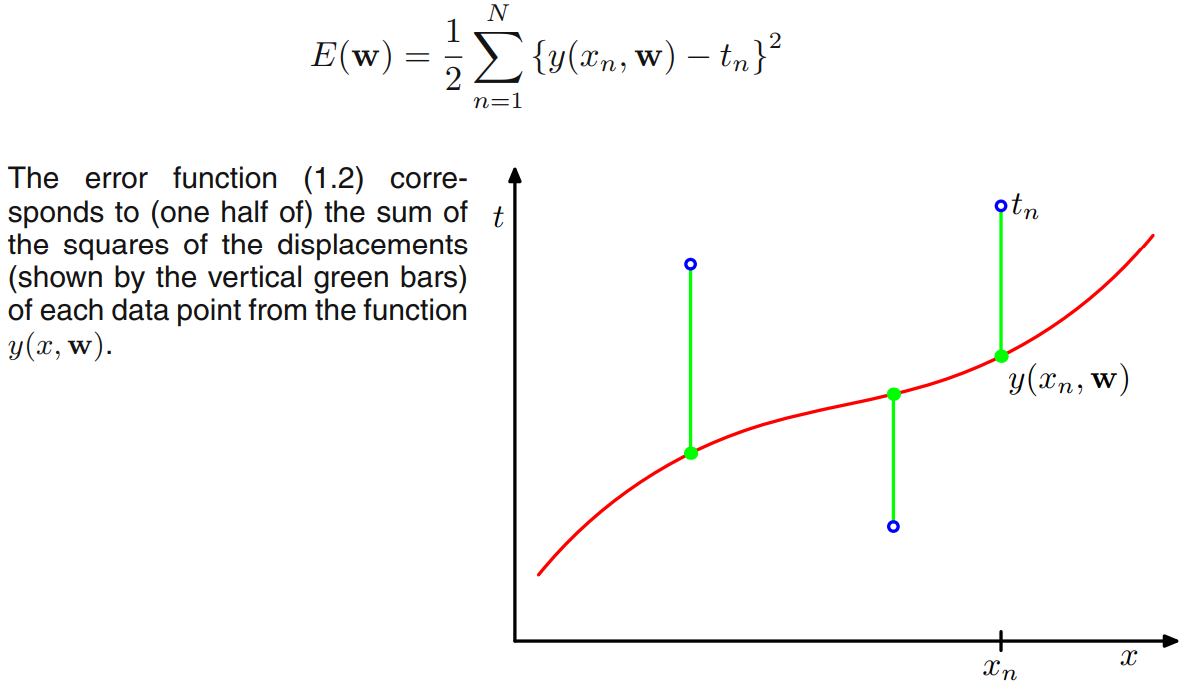
\includegraphics[width=0.80\textwidth]{plot_cost}
  		\caption{ Cost function for continuous type variables }
    \label{plot_cost_function}
 \end{figure}
\end{frame}

\begin{frame}{Curve fitting approach - Intuition about solving the problem}
We can solve the curve fitting problem by choosing the value of w for which
E(w) is as small as possible. Because the error function is a quadratic function of
the coefficients w, its derivatives with respect to the coefficients will be linear in the
elements of w, and so the minimization of the error function has a unique solution,
denoted by w$*$, which can be found in closed form. The resulting polynomial is
given by the function y(x, w$*$).
\end{frame}

\subsection{Learning algorithm}
\begin{frame}{Curve fitting approach - Gradient Descent}
\begin{figure}
  \centering
    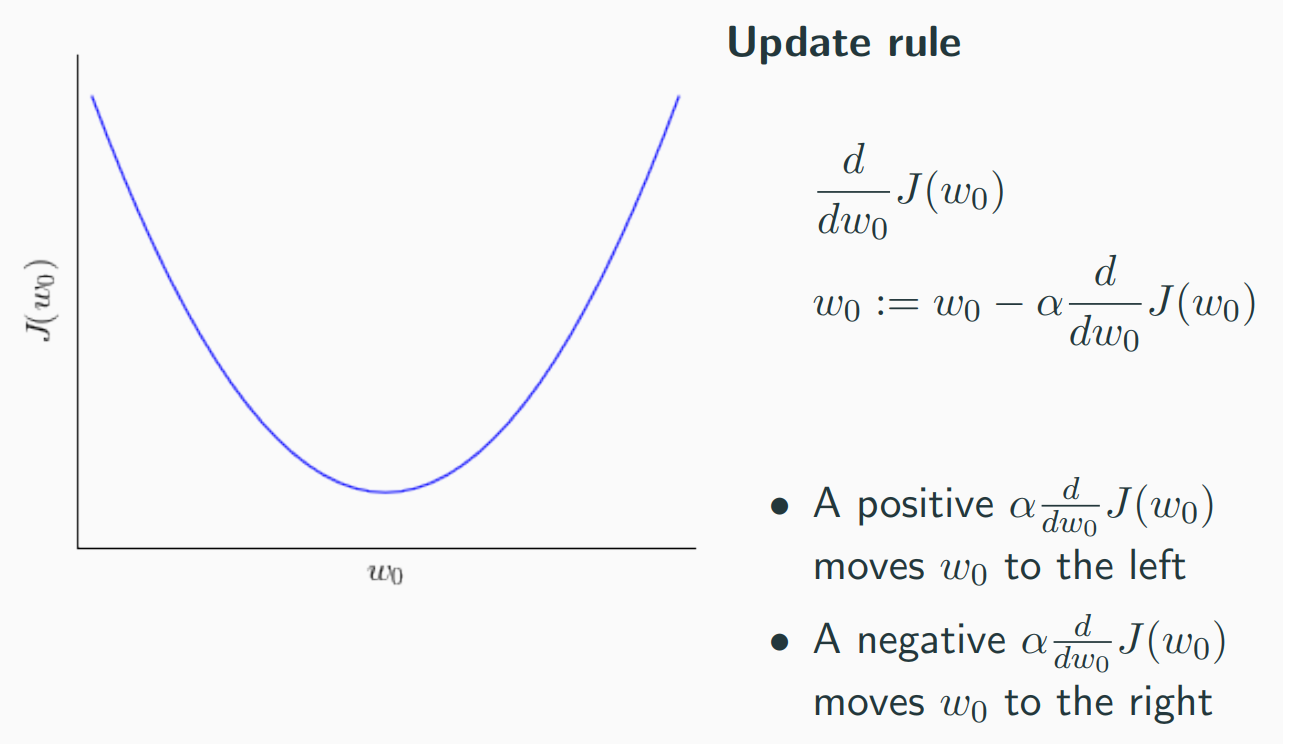
\includegraphics[width=0.85\textwidth]{updaterule}
  		\caption{ Gradient descent }
    \label{updaterule}
 \end{figure}
\end{frame}

\begin{frame}{BGD, SGD}
Batch gradient descent
\end{frame}

\begin{frame}{BGD, SGD}
Stochastic gradient descent
\end{frame}

\subsection{Gradient Descent - Multiple Regression problem}
\begin{frame}{Gradient Descent - Multiple Regression problem}
\begin{figure}
  \centering
    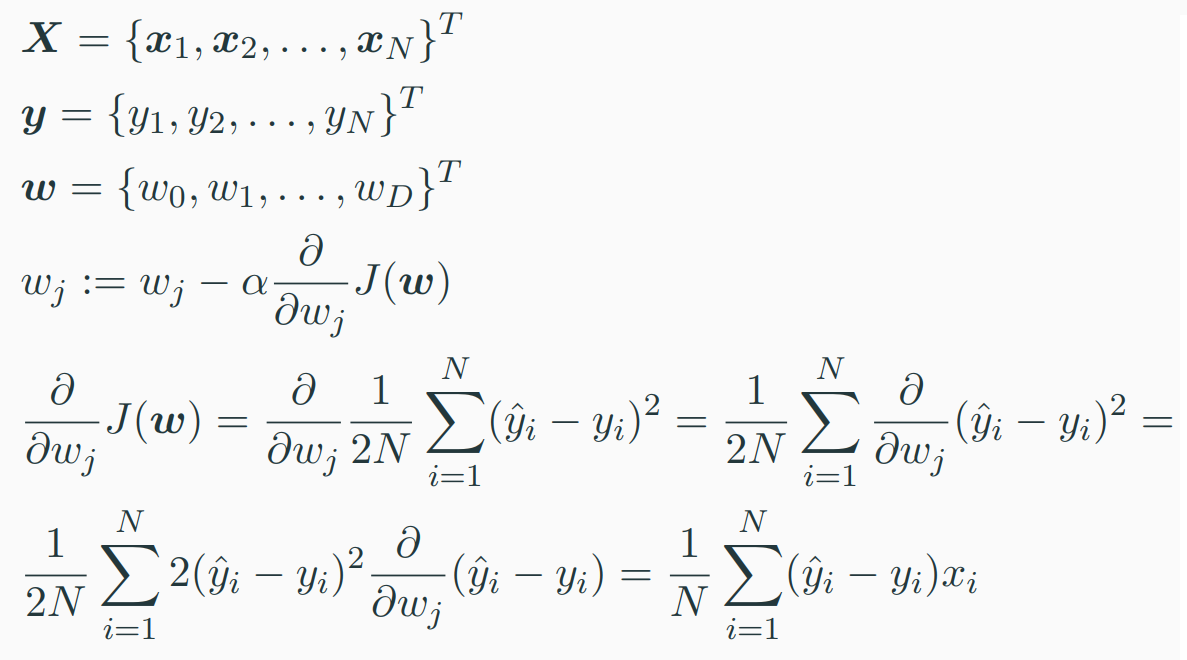
\includegraphics[width=0.65\textwidth]{gradientdescentmultipleregression}
  		\caption{ Multiple parameters increase the dimensionality of the parameters' vector }
    \label{gradientdescentmultipleregression}
 \end{figure}
\end{frame}

\begin{frame}{Curve fitting approach - How many features$?$}
\begin{figure}
  \centering
    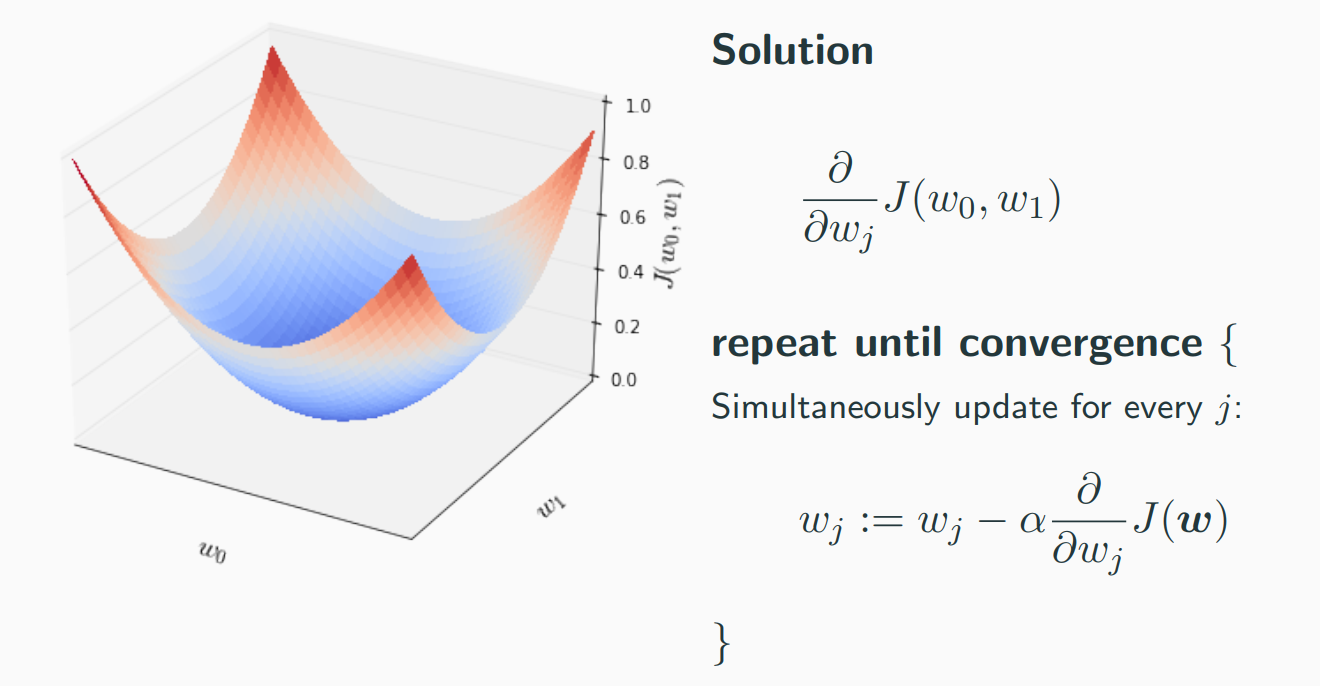
\includegraphics[width=0.85\textwidth]{twoparametercostfunction}
  		\caption{ Multi-dimensional cost function }
    \label{twoparametercostfunction}
 \end{figure}
\end{frame}

\begin{frame}{Curve fitting approach - How many features$?$}
Solve the problem using different dimensionalities for x
\begin{figure}
  \centering
    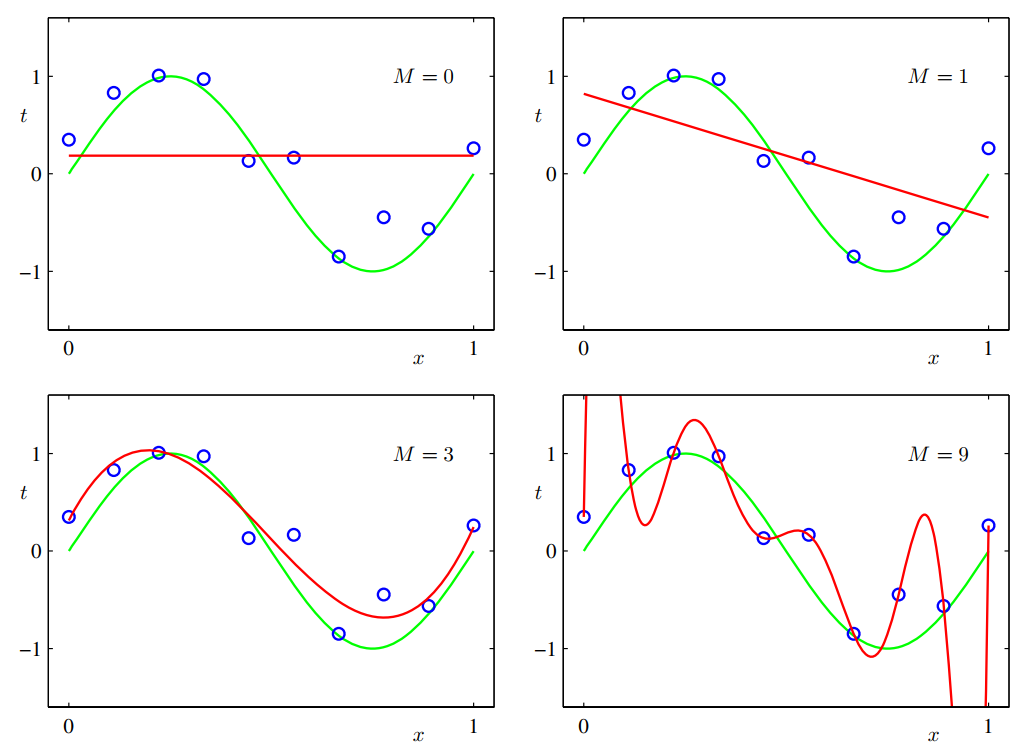
\includegraphics[width=0.55\textwidth]{howmanyfeatures}
  		\caption{ Multi-dimensional cost function }
    \label{howmanyfeatures}
 \end{figure}
\end{frame}

\begin{frame}{ Curve fitting approach - Addressing overfitting (variance) and underfitting (bias) }
Which is the correct number of features to be used$?$
\begin{figure}
  \centering
    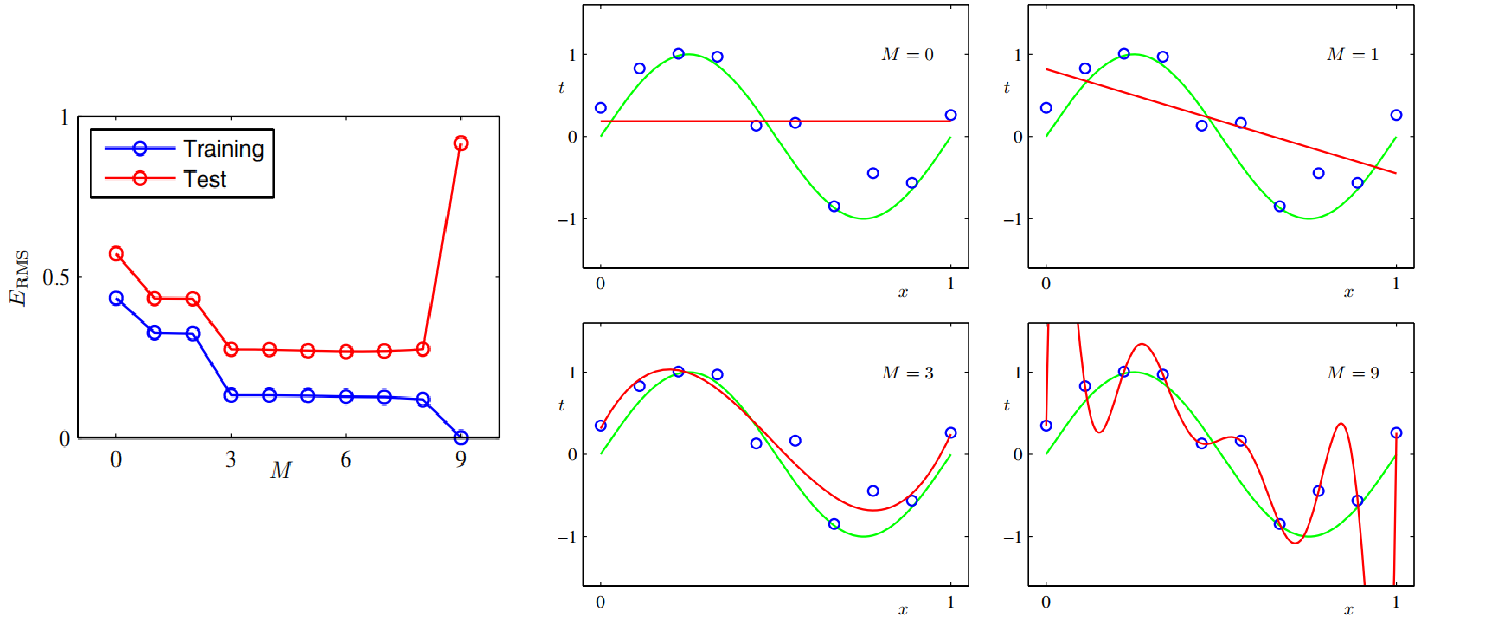
\includegraphics[width=0.85\textwidth]{performance}
  		\caption{ Diagnosing Overfitting and underfitting }
    \label{performance}
 \end{figure}
\end{frame}

\begin{frame}{ Curve fitting approach - Addressing overfitting (variance) and underfitting (bias) }
\begin{figure}
  \centering
    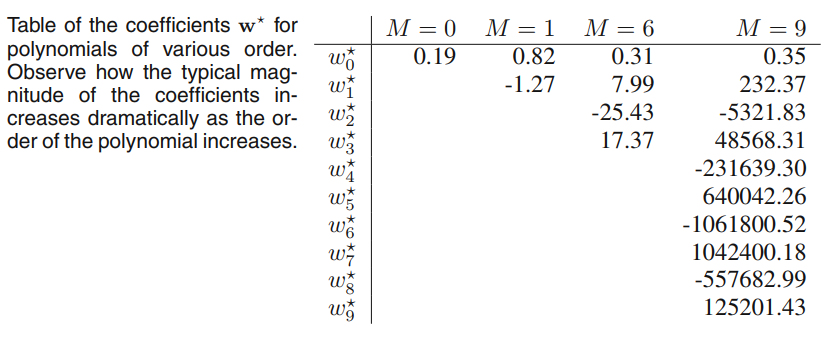
\includegraphics[width=0.85\textwidth]{whyoverunderfit}
  		\caption{ Why overfitting and underfitting$?$ }
    \label{performance}
 \end{figure}
\end{frame}

\begin{frame}{ Curve fitting approach - Causes of Overfitting }
\begin{itemize}
\item Extensive search in hypothesis 
\item Too many features (curse of dimensionality)
\item Insufficient examples
\end{itemize}
\end{frame}

\begin{frame}{ Curve fitting approach - Causes of Underfitting }
\begin{itemize}
\item Not enough data points
\item Not enough features 
\item Not enough polynomial terms to capture non-linearity
\end{itemize}
\end{frame}

\begin{frame}{ Curve fitting approach - Solve overfitting underfitting with regularization }
 \begin{figure}
  \centering
    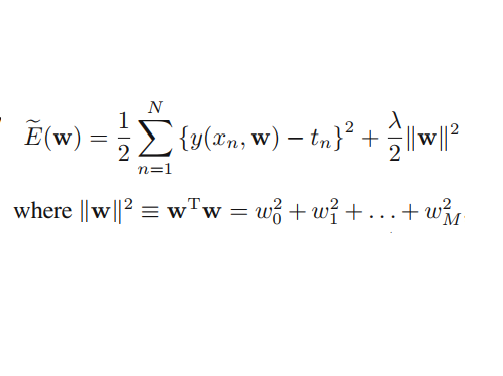
\includegraphics[width=0.8\textwidth]{regularization}
  		\caption{ Modified cost function }
    \label{regularization}
 \end{figure}
\end{frame}

\begin{frame}{ Curve fitting approach - Solve overfitting underfitting with regularization }
 \begin{figure}
  \centering
    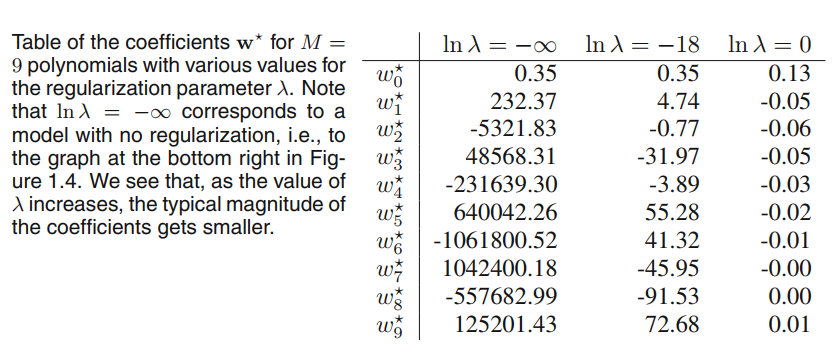
\includegraphics[width=0.8\textwidth]{tablereg}
  		\caption{ Learning parameters after applying regularization }
    \label{tablereg}
 \end{figure}
\end{frame}

\begin{frame}{ Curve fitting approach - Solve overfitting underfitting with regularization }
 \begin{figure}
  \centering
    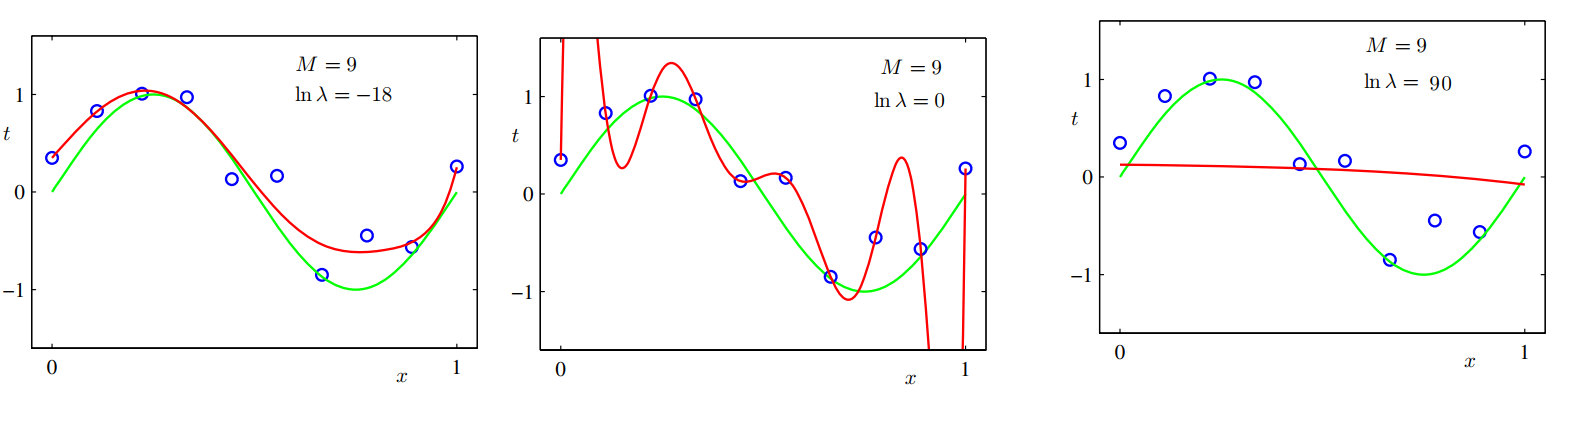
\includegraphics[width=1.0\textwidth]{applyingreg}
  		\caption{ Apllying regularization }
    \label{tablereg}
 \end{figure}
\end{frame}

\begin{frame}{ Curve fitting approach - Solve overfitting underfitting adding more data (always works) }
 \begin{figure}
  \centering
    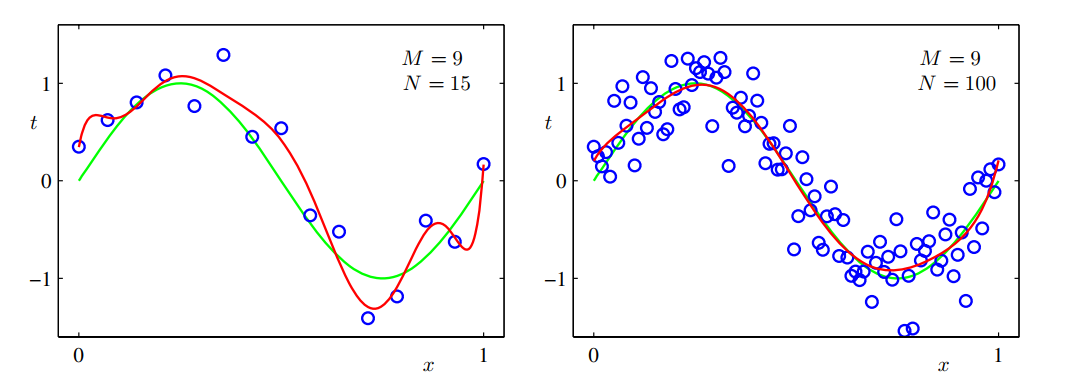
\includegraphics[width=1.1\textwidth]{moredata}
  		\caption{ The more data, the better }
    \label{tablereg}
 \end{figure}
\end{frame}

%%%%%%%%%%%%%%%%%%%%%%%%%%%%%%%%%%%%%Multivariate linear regression%%%%%%%%%%%%%%%%%%%%%%%%%%%%%%%%%%%%%%%

\subsection{Summary}
\begin{frame}{Summary}
\begin{itemize}
\setlength\itemsep{2em}
\item Hypothesis
\item Cost function
\item Learning algorithm
\end{itemize}
\end{frame}

\begin{frame}{Summary - Hyperparameters}
Hyperparameters:

\end{frame}

\section{References}
\begin{frame}{References I}
\begin{itemize}
\item Olivier Bousquet and L´eon Bottou, The tradeoffs of large scale learning, Advances in Neural Information Processing Systems 20 (J. C. Platt, D. Koller, Y. Singer, and S. T. Roweis, eds.), Curran Associates, Inc., 2008, pp. 161–168.

\item Christopher M. Bishop, Pattern recognition and machine learning (information science and statistics), Springer-Verlag New York, Inc., Secaucus, NJ, USA, 2006.

\item Peter Flach, Machine learning: The art and science of algorithms that make sense of data, Cambridge University Press, New York, NY, USA, 2012.

\item Geoffrey Hinton, Csc321: Introduction to neural networks and
machine learning, University Lecture, 2014.
\end{itemize}
\end{frame}

\begin{frame}{References II}
\begin{itemize}
\item Thomas M. Mitchell, Machine learning, 1 ed., McGraw-Hill, Inc., New York, NY, USA, 1997.

\item Kevin P. Murphy, Machine learning: A probabilistic perspective, The MIT Press, 2012.

\item Andrew Ng, Note 1, Lecture notes in CS 229 Machine Learning, 2012.

%\item Jason W. Osborne and Elaine Waters, Four assumptions of multiple regression that researchers should always test, Practical Assessment Research and Evaluation 8 (2002), no. 2.

\end{itemize}
\end{frame}


\end{document}
